% ============================================================================
\section{Applications and frontier topics}
% ============================================================================

\begin{frame}{The 2026 TTS Landscape}
  \begin{itemize}\itemsep0.4em\footnotesize
    \item \textbf{Flow matching won the acoustic model:} F5-TTS and CosyVoice-class systems generate speech features non-autoregressively in a few ODE steps, with zero-shot cloning from a short reference clip.
    \item \textbf{Codec language models power conversation:} end-to-end voice modes speak through speech tokens directly, with no separate TTS stage.
    \item \textbf{Downloadable weights closed much of the gap:} XTTS, F5-TTS, and Kokoro all run locally, but check the licence before shipping: Kokoro is Apache-2.0, while the XTTS and F5-TTS checkpoints are non-commercial. Commercial systems (ElevenLabs, OpenAI, Google) still lead on expressiveness and robustness.
    \item Remaining hard problems: long-form consistency, fine-grained emotion control, low-resource languages, and singing.
  \end{itemize}
\end{frame}

\begin{frame}{Example: F5-TTS}
  \begin{itemize}\footnotesize\itemsep0.2em
    \item Text characters (padded with filler tokens) and a masked mel-spectrogram enter diffusion-transformer blocks; the model learns a flow from noise to the missing speech, conditioned on text and the audio prompt.
    \item Zero-shot cloning falls out of infilling, the same idea as Voicebox, with a simpler pipeline: no phonemizer, no duration model, no forced aligner.
  \end{itemize}
  \centering
  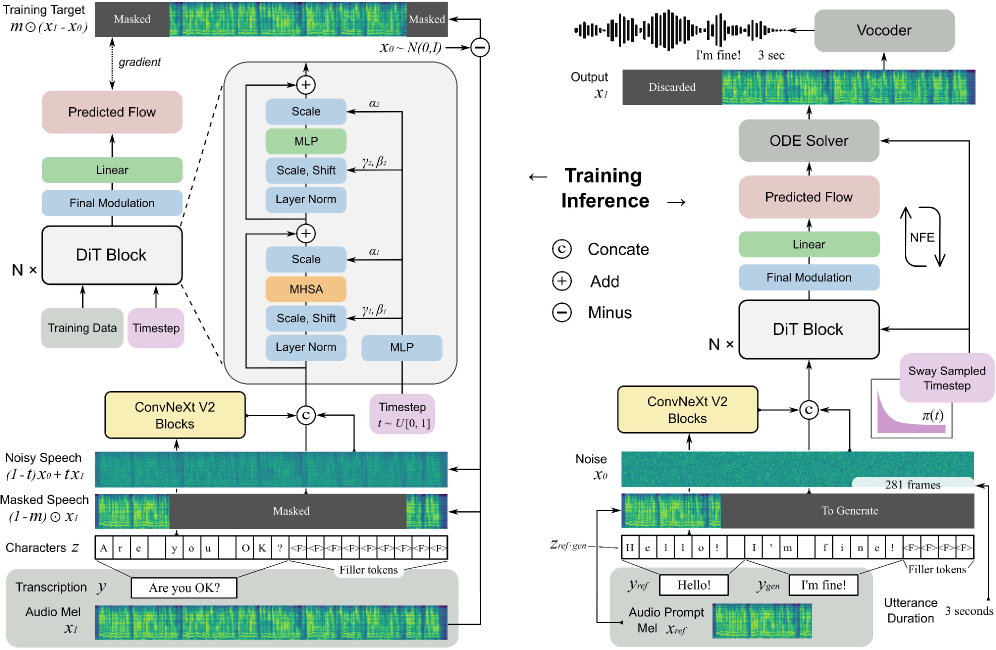
\includegraphics[width=0.7\textwidth,height=0.52\textheight,keepaspectratio]{images/tts/f5tts_flow_matching_architecture.png}\\[0.15em]
  {\scriptsize F5-TTS training (left) and inference (right). Chen et al., ``F5-TTS: A Fairytaler that Fakes Fluent and Faithful Speech with Flow Matching,'' \href{https://arxiv.org/abs/2410.06885}{arXiv:2410.06885}, Figure 1.}
\end{frame}

\begin{frame}{TTS in Real-Time Voice Agents}
  \begin{itemize}\itemsep0.5em
    \item A voice agent chains streaming ASR, an LLM, and TTS; the user hears silence until the first audio chunk arrives, so \textbf{time to first audio} matters more than total synthesis time.
    \item \textbf{Streaming synthesis:} start speaking while the LLM is still writing, chunking at sentence or phrase boundaries; codec-LM stacks can stream token by token.
    \item \textbf{Barge-in:} users interrupt mid-sentence; the stack must stop playback, flush queued audio, and hand the conversation back to the LLM.
    \item Expressive control is moving from Speech Synthesis Markup Language (SSML) tags toward natural-language style prompts (``speak warmly, a little slower'').
  \end{itemize}
\end{frame}
